\fontsize{9}{10.5}\selectfont

\par\Needspace{120pt}\medskip
\section*{Paper 7: AY2025/\allowbreak{}26 Semester 1 --- Smart Home Control System}\label{paper-2526-s1}
\phantomsection\addcontentsline{toc}{section}{Paper 7: AY2025/26 Semester 1 --- Smart Home Control System}\markboth{AY2025/26 S1}{}
\sectionlabel{h-191-ay202526-semester-1--smart-home-control-system}
\textbf{Source:} \href{run:/Users/bryangoh/Work/ntu-cs/sc2006/pyps/SC2006\_AY2526\_S1\_Questions.pdf}{Question paper}, Q1--Q4 on PDF pp. 1--3; Appendix A on p. 4.




\begin{studycolumns}
\vspace{0pt}
\textbf{Case facts.} Owners control lights, AC and door locks through a mobile app or LLM-powered voice assistant. The assistant interprets voice requests and can ask clarifying questions. Owners grant/\allowbreak{}revoke temporary guest access to specific doors. Guests may lock/\allowbreak{}unlock only during their permitted period; denied out-of-window attempts are logged. Administrators manage accounts, credentials and access rights but do not control devices. All guest-access activity is logged.

\needspace{4\baselineskip}
\subsection*{Q1 --- Use cases (25 marks)}
\sectionlabel{h-q1--use-cases-25-marks-5}
\textbf{(a) Actors/\allowbreak{}use cases/\allowbreak{}relationships (18). (b) Guest door-access description (7).}


\textbf{(a)} Actors: Homeowner, Guest, Administrator and external controlled devices (Lights, AC, Door Locks). App and voice assistant are interfaces/\allowbreak{}components of the SHCS, not additional human users. An external hosted speech/\allowbreak{}LLM service can be a supporting actor if that deployment boundary is chosen, but hosting is not specified in this appendix.
\end{studycolumns}


\par\smallskip\noindent\begin{minipage}{\linewidth}\centering
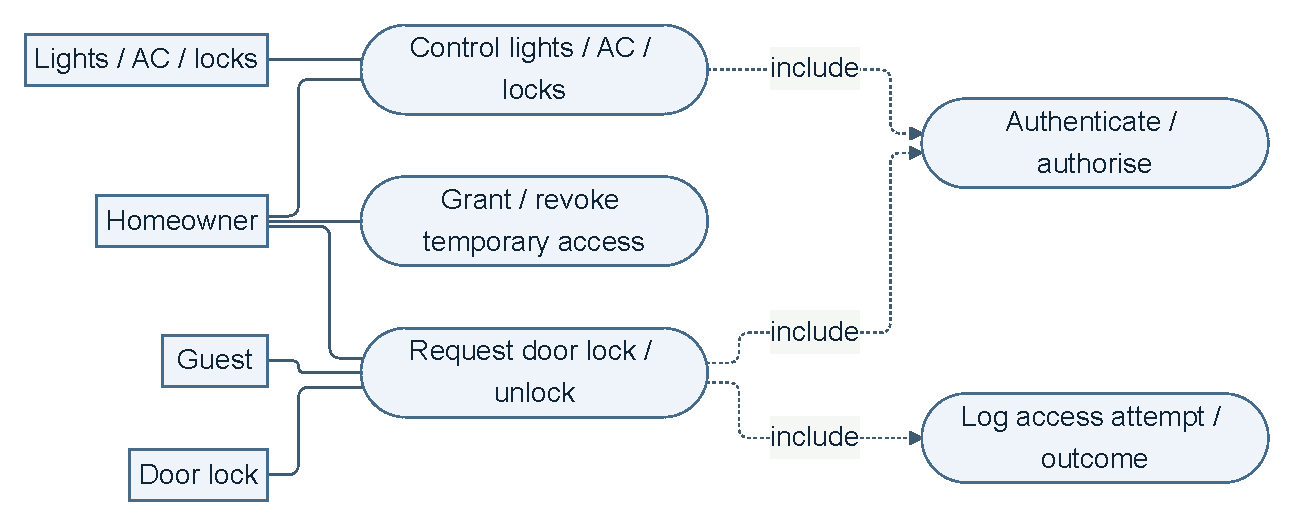
\includegraphics[width=364.32pt]{images/fig-079-user.pdf}
\captionof{figure}{Q1 --- Use cases (25 marks) --- device control and access}\end{minipage}\par\smallskip


\par\smallskip\noindent\begin{minipage}{\linewidth}\centering
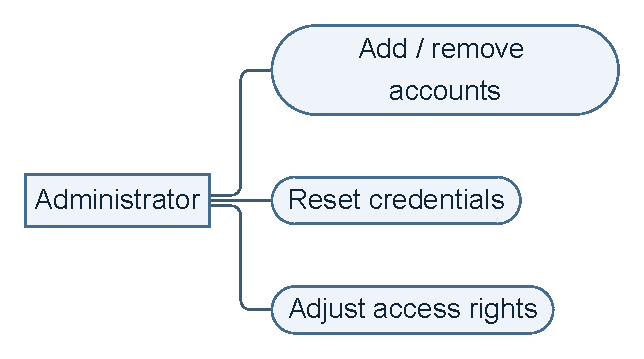
\includegraphics[width=181.28pt]{images/fig-079-admin.pdf}
\captionof{figure}{Q1 --- Use cases (25 marks) --- account administration}\end{minipage}\par\smallskip



\par\smallskip\noindent\begin{minipage}{\linewidth}\centering
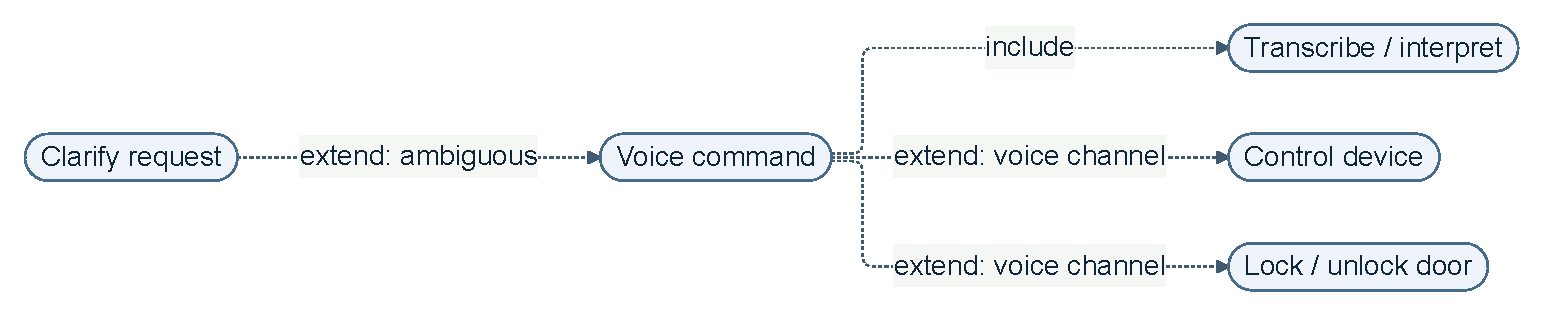
\includegraphics[width=434.72pt]{images/fig-079-voice.pdf}
\captionof{figure}{Q1 --- Use cases (25 marks) --- optional voice channel and clarification}\end{minipage}\par\smallskip

\begin{studycolumns}
\vspace{0pt}




Authorisation includes a guest's door-specific grant, revocation status and current time. Do not generalise Administrator from Homeowner or give administrators device-control associations. An owner-granted access period is not a one-time login token or permission for every door. Both permitted and denied guest attempts must reach the log.

\textbf{(b) Use case: Guest Door Access.} Primary actor: Guest. Supporting actor: Door Lock; voice interface if selected. Preconditions: guest identity can be authenticated; door and guest grant can be identified. Do \textbf{not} require ``current time is valid'' as the only precondition if the description must cover out-of-window denial. Flow: guest requests lock/\allowbreak{}unlock for a specific door through app or voice; system interprets/\allowbreak{}clarifies the request as needed; authenticate guest; check action, door, grant, revocation and time; execute permitted command through the lock interface; record request/\allowbreak{}time/\allowbreak{}outcome and show confirmation. Alternatives: no grant, revoked grant, wrong door or outside period, deny and log; ambiguous command, clarify without unlocking; device failure, log failure and report it rather than claiming success. A voice utterance alone is not proof of identity.

\needspace{4\baselineskip}
\subsection*{Q2 --- Access states, voice activity and process (25 marks)}
\sectionlabel{h-q2--access-states-voice-activity-and-process-25-marks}
\textbf{(a) Temporary guest access-controller state machine (4). (b) Guest voice-unlock activity/\allowbreak{}swimlanes (8). (c) Waterfall/\allowbreak{}Agile comparison: flexibility, customer involvement, delivery and one advantage each (5). (d) Two sprint advantages and two challenges, with examples (8).}


\textbf{(a)} Model one guest--door grant. \textbf{Assumption:} a time window is half-open \code{[start,\allowbreak{}end)}; the paper requires a strict window but does not specify endpoint inclusion. Agree the exact policy before implementation/\allowbreak{}testing.
\end{studycolumns}


\par\smallskip\noindent\begin{minipage}{\linewidth}\centering
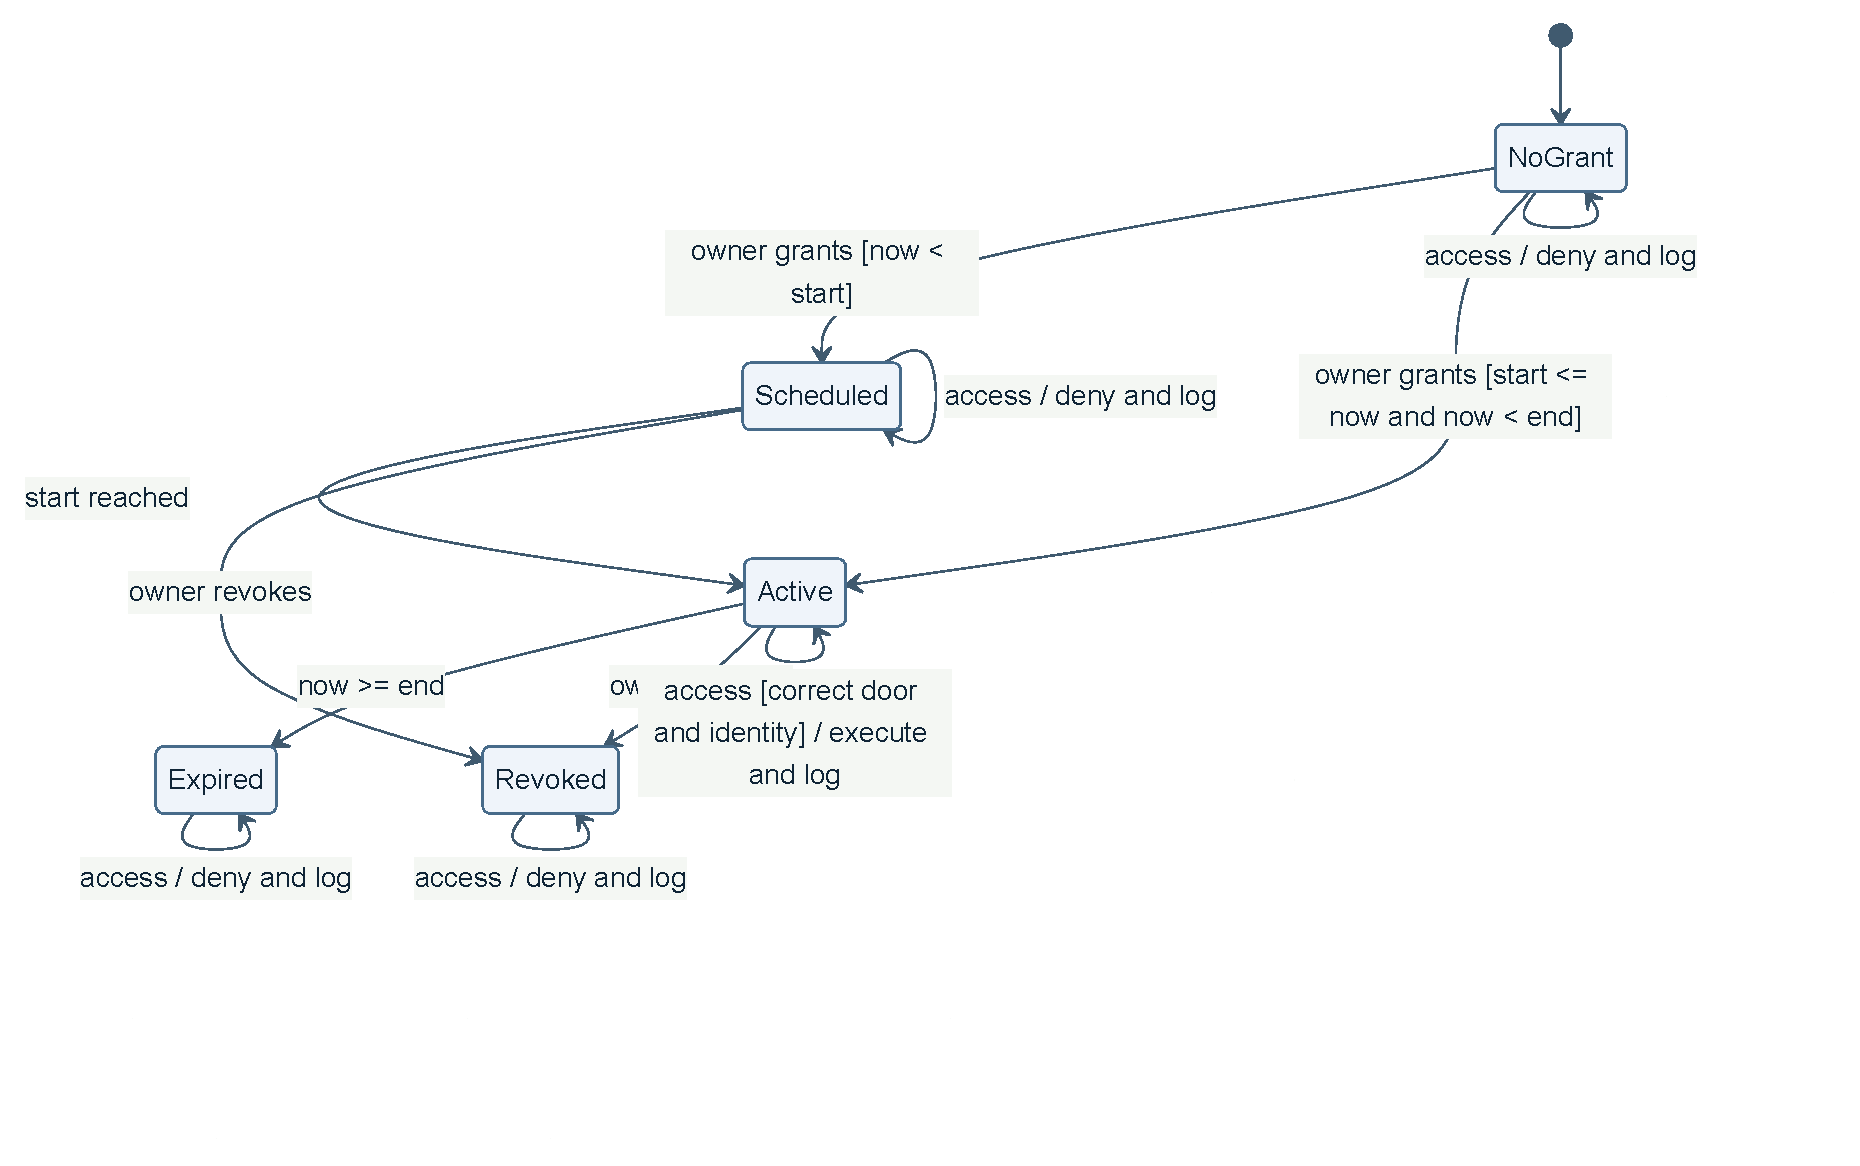
\includegraphics[width=446.65pt]{images/fig-080.pdf}
\captionof{figure}{Q2 --- Access states, voice activity and process (25 marks)}\end{minipage}\par\smallskip


A new grant can create a fresh controller/\allowbreak{}grant instance. A command arriving late must recheck time before execution; being previously Active is not enough.





\textbf{(b)}


\par\smallskip\noindent\begin{minipage}{\linewidth}\centering
{\scriptsize\textbf{Interpret and clarify}}\par\smallskip
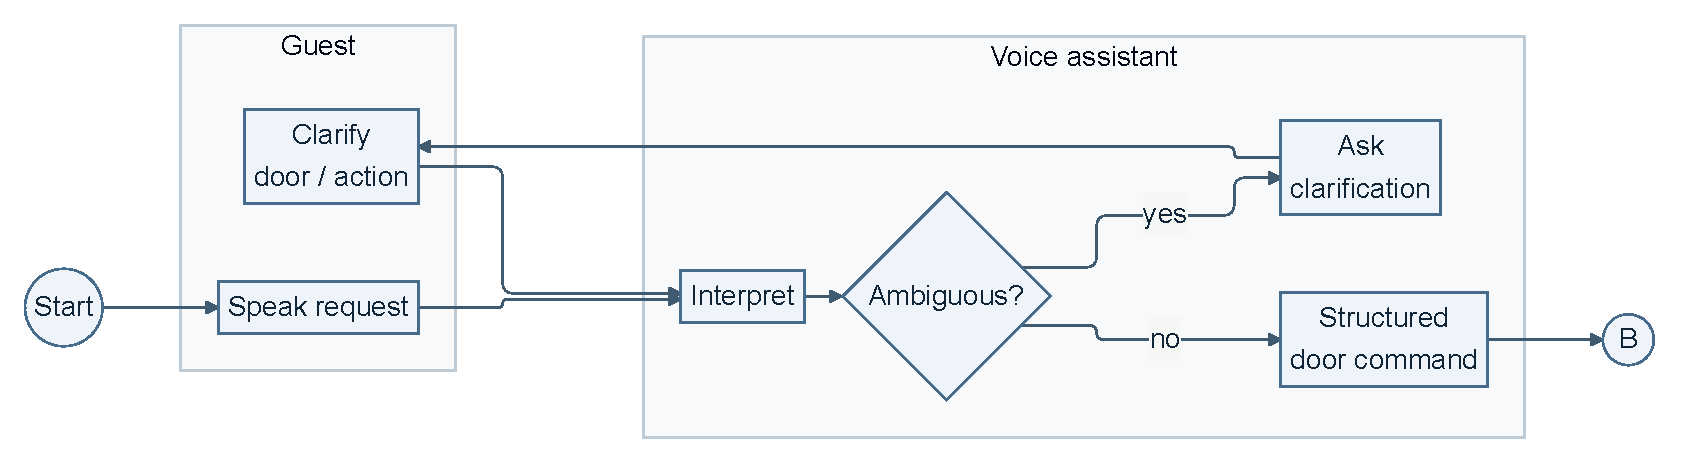
\includegraphics[width=430.00pt]{images/fig-081-a.pdf}\par\smallskip
{\scriptsize\textbf{Enforce policy, operate lock, log result}}\par\smallskip
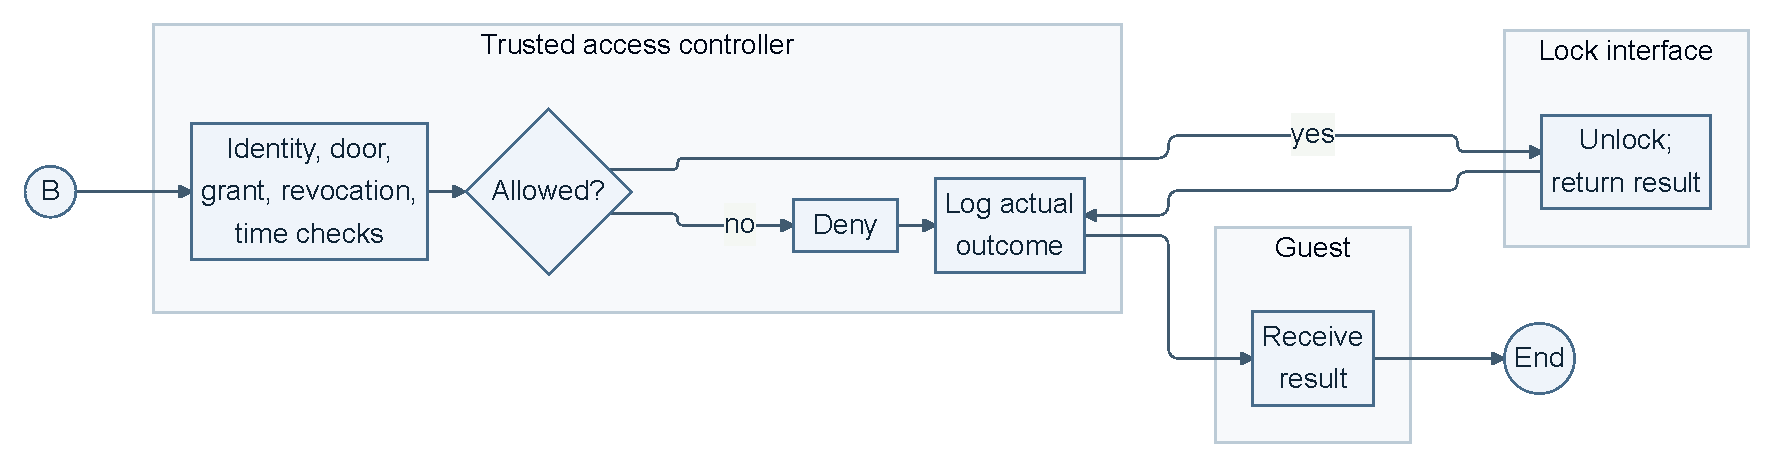
\includegraphics[width=454.00pt]{images/fig-081-b.pdf}\par\smallskip
\captionof{figure}{Q2 --- Access states, voice activity and process (25 marks)}\end{minipage}\par\smallskip

\begin{studycolumns}
\vspace{0pt}










LLM output proposes an action; deterministic access rules decide whether it can occur. Failure to interpret/\allowbreak{}authenticate must not unlock the door.

\textbf{(c)} Compare flexibility, customer involvement, delivery and strengths using \hyperref[answer-waterfall]{W, p.\ \pageref{answer-waterfall}}. Apply the comparison to owner/guest/device access increments.

\textbf{(d)} Apply \hyperref[answer-scrum]{S, p.\ \pageref{answer-scrum}}. Two benefits: owner feedback on voice clarification; visible tested guest-access increments. Two challenges: oversized voice/device work (split/spike) and hardware/urgent-change dependencies (doubles, early integration and backlog negotiation).

\needspace{4\baselineskip}
\subsection*{Q3 --- Smart-home architecture and pattern judgement (25 marks)}
\sectionlabel{h-q3--smart-home-architecture-and-pattern-judgement-25-marks}
\textbf{(a)(i) Architecture/\allowbreak{}detailed classes (8); (ii) one NFR and alternative architecture (8). (b)(i) Combined-pattern scenario/\allowbreak{}classes (6); (ii) evaluate the cost of pattern overuse (3).}


\textbf{(a)(i)} Use layered channel interfaces, application command control, domain access policy and device gateways. Both app and voice requests reach the same trusted policy before actuation.
\end{studycolumns}


\par\smallskip\noindent\begin{minipage}{\linewidth}\centering
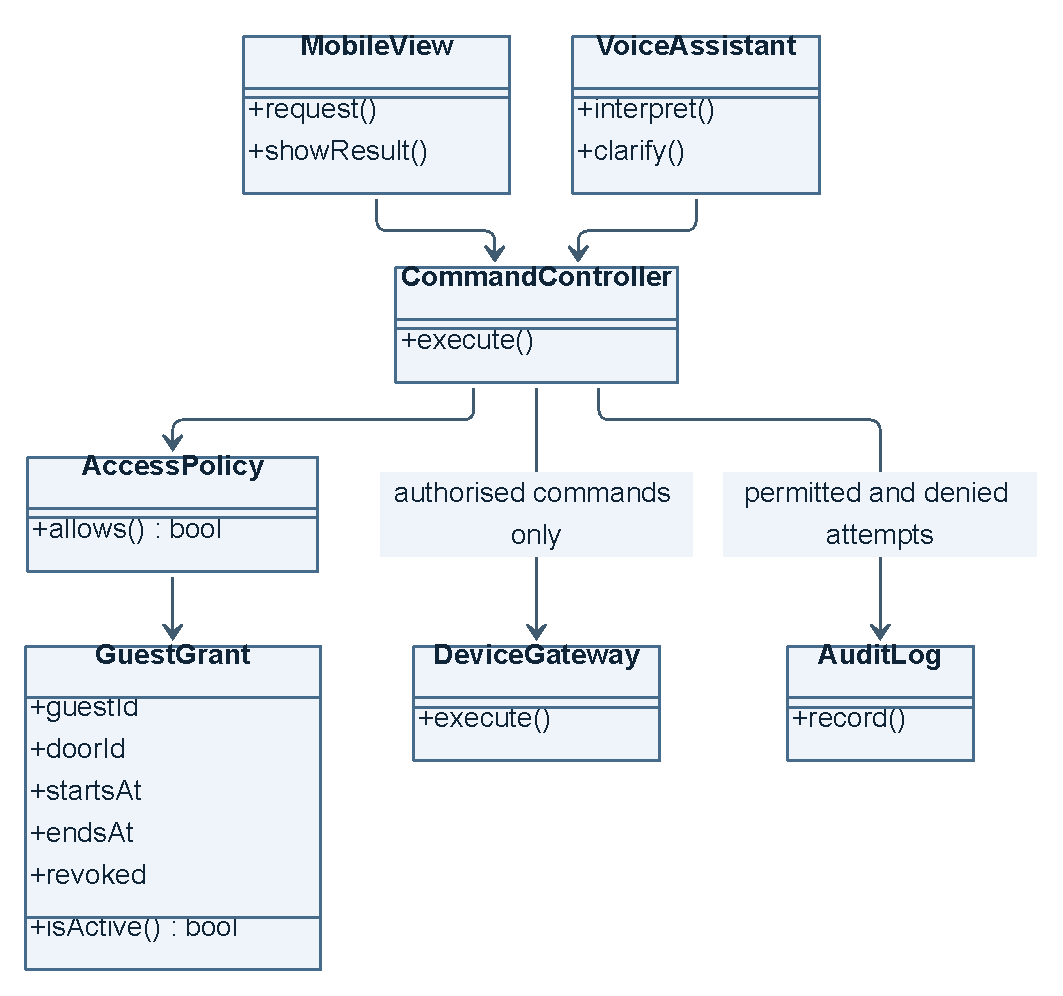
\includegraphics[width=298.90pt]{images/fig-082.pdf}
\captionof{figure}{Q3 --- Smart-home architecture and pattern judgement (25 marks)}\end{minipage}\par\smallskip




\textbf{(a)(ii)} Choose \textbf{security}, explicitly required by authentication, role separation and time-limited door grants. An alternative \textbf{client--server architecture with a security Facade/\allowbreak{}reference gate} treats app and LLM processing as untrusted input channels. Only a trusted server-side access service can invoke device gateways. Account administration uses a separate authorised API and does not confer device-control rights.




\par\smallskip\noindent\begin{minipage}{\linewidth}\centering
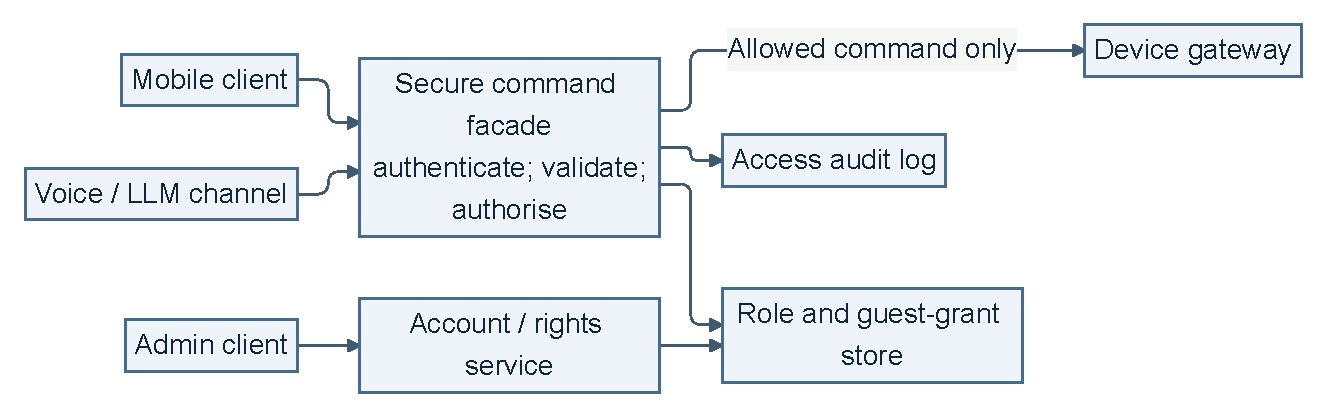
\includegraphics[width=374.00pt]{images/fig-083.pdf}
\captionof{figure}{Q3 --- Smart-home architecture and pattern judgement (25 marks)}\end{minipage}\par\smallskip

\begin{studycolumns}
\vspace{0pt}



Compared with policy spread among clients, a central gate prevents channel-specific bypasses and keeps one authoritative time/\allowbreak{}grant check. It introduces connectivity/\allowbreak{}availability concerns that require explicit failure behaviour; door access must not silently bypass checks when the policy service fails. This is a deployment/\allowbreak{}trust-boundary alternative compatible with layered internals.

\textbf{(b)(i)} Combine Strategy for role-specific permission policies with Simple Factory for selecting the policy from the \textbf{authenticated role}, never an LLM-supplied role string.





\textbf{Class diagram:} use \hyperref[shared-pattern]{P, p.\ \pageref{shared-pattern}}. Context = \code{Access\allowbreak{}Service}; Strategy = \code{Access\allowbreak{}Policy}; Factory = \code{Policy\allowbreak{}Factory}. Concrete strategies: \code{Owner\allowbreak{}Policy}, \code{Guest\allowbreak{}Policy}, \code{Administrator\allowbreak{}Policy}. Interface/concrete operations: \code{allows()}. Select from the authenticated role, never an LLM role string. Guest checks door/time/revocation; Administrator denies device control.







\textbf{(b)(ii)} Agree: use \hyperref[answer-pattern-cost]{C, p.\ \pageref{answer-pattern-cost}}. Trivial access rules may need only a policy table; introduce patterns for actual policy variation/coupling.

\needspace{4\baselineskip}
\subsection*{Q4 --- User inputs and automation (25 marks)}
\sectionlabel{h-q4--user-inputs-and-automation-25-marks}
\textbf{(a)(i) Derive ECs for Name, Phone Number, Access Expiry Date and Type of the User (4). (ii) Give on/\allowbreak{}below/\allowbreak{}above boundary values (4). (iii) Design defensive tests (5).}


\textbf{Input interpretation.} Name must be ASCII; Phone Number is a 8-digit integer; Access Expiry Date is between 2025 and 2030; Type of the User is one of \code{Administrator}, \code{Owner}, \code{Guest}, \code{One Time User}. Assume a positive 8-digit numeric value (not a string whose leading zeroes count as digits), inclusive complete calendar years, and one-day date resolution. These interpretations are stated because the brief does not specify parsing details. Do not invent an ASCII-field length limit.

\textbf{(i) Equivalence classes:}
\end{studycolumns}


{\fontsize{8.5}{9.8}\selectfont
\begin{longtable}{L{\dimexpr 0.21857\linewidth-5.25pt\relax}L{\dimexpr 0.33977\linewidth-8.15pt\relax}L{\dimexpr 0.44166\linewidth-10.60pt\relax}}
\toprule
\rowcolor{ice}\textbf{Field} & \textbf{Valid EC} & \textbf{Invalid ECs} \\
\midrule\endfirsthead
\toprule\rowcolor{ice}\textbf{Field} & \textbf{Valid EC} & \textbf{Invalid ECs} \\
\midrule\endhead
\multicolumn{3}{r}{\scriptsize Continued on next page}\\\endfoot
\bottomrule\endlastfoot
Name & ASCII text & Text containing non-ASCII characters \\
Phone Number & Integer 10000000\ldots{}99999999 & Integer below 10000000; integer above 99999999; malformed/\allowbreak{}non-integer input at the input boundary \\
Access Expiry Date & Real calendar date 2025-01-01\ldots{}2030-12-31 & Real date before 2025-01-01; real date after 2030-12-31; malformed/\allowbreak{}nonexistent date \\
Type of the User & One EC containing \{Administrator, Owner, Guest, One Time User\} & Any unlisted value \\
\end{longtable}
}

The category set is \textbf{one valid EC}, although testing all its few members is useful. No empty-string prohibition or printable-only ASCII restriction is supplied; clarify those separately instead of asserting an invented oracle.

\textbf{(ii) Boundary triplets:}




{\fontsize{8.5}{9.8}\selectfont
\begin{longtable}{L{\dimexpr 0.27995\linewidth-8.96pt\relax}L{\dimexpr 0.23807\linewidth-7.62pt\relax}L{\dimexpr 0.24099\linewidth-7.71pt\relax}L{\dimexpr 0.24099\linewidth-7.71pt\relax}}
\toprule
\rowcolor{ice}\textbf{Field /\allowbreak{} boundary} & \textbf{Just below} & \textbf{On boundary} & \textbf{Just above} \\
\midrule\endfirsthead
\toprule\rowcolor{ice}\textbf{Field /\allowbreak{} boundary} & \textbf{Just below} & \textbf{On boundary} & \textbf{Just above} \\
\midrule\endhead
\multicolumn{4}{r}{\scriptsize Continued on next page}\\\endfoot
\bottomrule\endlastfoot
Phone Number: minimum & 9999999 (reject) & 10000000 (accept) & 10000001 (accept) \\
Phone Number: maximum & 99999998 (accept) & 99999999 (accept) & 100000000 (reject) \\
Access Expiry Date: earliest & 2024-12-31 (reject) & 2025-01-01 (accept) & 2025-01-02 (accept) \\
Access Expiry Date: latest & 2030-12-30 (accept) & 2030-12-31 (accept) & 2031-01-01 (reject) \\
\end{longtable}
}

ASCII membership and unordered categories have no specified application-level ordered boundary. Malformed values are additional EC tests, not numeric/\allowbreak{}date neighbours.

\textbf{(iii) Defensive suite.} Use the common testing conventions below; valid rows combine boundaries, invalid rows isolate one field. The full boundary suite is retained.




{\fontsize{8.5}{9.8}\selectfont
\begin{longtable}{L{\dimexpr 0.16951\linewidth-6.78pt\relax}L{\dimexpr 0.16951\linewidth-6.78pt\relax}L{\dimexpr 0.17251\linewidth-6.90pt\relax}L{\dimexpr 0.17980\linewidth-7.19pt\relax}L{\dimexpr 0.30866\linewidth-12.35pt\relax}}
\toprule
\rowcolor{ice}\textbf{Name} & \textbf{Phone Number} & \textbf{Access Expiry Date} & \textbf{Type of the User} & \textbf{Expected /\allowbreak{} purpose} \\
\midrule\endfirsthead
\toprule\rowcolor{ice}\textbf{Name} & \textbf{Phone Number} & \textbf{Access Expiry Date} & \textbf{Type of the User} & \textbf{Expected /\allowbreak{} purpose} \\
\midrule\endhead
\multicolumn{5}{r}{\scriptsize Continued on next page}\\\endfoot
\bottomrule\endlastfoot
\code{Alex} & \code{10000000} & \code{2025-\allowbreak{}01-\allowbreak{}01} & \code{Administrator} & Accept --- valid boundaries /\allowbreak{} category coverage \\
\code{Alex} & \code{10000001} & \code{2025-\allowbreak{}01-\allowbreak{}02} & \code{Owner} & Accept --- valid boundaries /\allowbreak{} category coverage \\
\code{Alex} & \code{99999998} & \code{2030-\allowbreak{}12-\allowbreak{}30} & \code{Guest} & Accept --- valid boundaries /\allowbreak{} category coverage \\
\code{Alex} & \code{99999999} & \code{2030-\allowbreak{}12-\allowbreak{}31} & \code{One Time User} & Accept --- valid boundaries /\allowbreak{} category coverage \\
\code{Alex} & \code{54999999} & \code{2027-\allowbreak{}07-\allowbreak{}01} & \code{Administrator} & Accept --- interior baseline /\allowbreak{} category coverage \\
\code{caf\'{e}} & \code{54999999} & \code{2027-\allowbreak{}07-\allowbreak{}01} & \code{Administrator} & Reject --- non-ASCII Name \\
\code{Alex} & \code{9999999} & \code{2027-\allowbreak{}07-\allowbreak{}01} & \code{Administrator} & Reject --- Phone Number below minimum \\
\code{Alex} & \code{100000000} & \code{2027-\allowbreak{}07-\allowbreak{}01} & \code{Administrator} & Reject --- Phone Number above maximum \\
\code{Alex} & \code{54999999} & \code{2024-\allowbreak{}12-\allowbreak{}31} & \code{Administrator} & Reject --- Access Expiry Date below minimum \\
\code{Alex} & \code{54999999} & \code{2031-\allowbreak{}01-\allowbreak{}01} & \code{Administrator} & Reject --- Access Expiry Date above maximum \\
\code{Alex} & \code{54999999} & \code{2027-\allowbreak{}07-\allowbreak{}01} & \code{Unknown} & Reject --- unlisted Type of the User \\
\code{Alex} & \code{12x} & \code{2027-\allowbreak{}07-\allowbreak{}01} & \code{Administrator} & Reject --- malformed integer; extra defensive case \\
\code{Alex} & \code{54999999} & \code{2025-\allowbreak{}02-\allowbreak{}30} & \code{Administrator} & Reject --- nonexistent calendar date; extra defensive case \\
\end{longtable}
}

\begin{studycolumns}
\vspace{0pt}

The Q4 category \code{One Time User} is valid for this input question, although Appendix A does not define that role's device permissions. Do not invent its access policy from the category name.

\textbf{(b) How can LLMs assist automated testing? (4). (c) At least four challenges of fully automated development (8).}


\textbf{(b)} Use requirements and code context to propose tests, fixtures, boundary cases and automation scripts; run them through a real test runner and report actual results. Generate guest-access cases for wrong door, revocation and exact time edges, and validate expected results against the agreed policy. Review generated code/\allowbreak{}oracles and measure meaningful coverage. An LLM's claim that a test passed is not execution evidence; voice-language tests also need representative ambiguous/\allowbreak{}adversarial requests and repeatability controls.

\textbf{(c)} Four challenges with consequences: \textbf{ambiguous/\allowbreak{}incomplete requirements} require stakeholder clarification, otherwise correct-looking code solves the wrong problem; \textbf{incorrect or nondeterministic generation} can introduce defects/\allowbreak{}security flaws, requiring independent execution and review; \textbf{integration/\allowbreak{}context limits} make existing interfaces, hardware behaviour and cross-component invariants hard to preserve; \textbf{validation and accountability} require trusted oracles, quality-attribute evidence and responsibility for consequential decisions. Maintenance adds further difficulty because changes must preserve compatibility, intent and operational safety across versions. In this case, a plausible voice response cannot establish that a physical door was correctly authorised or operated.
\end{studycolumns}

\par\Needspace{120pt}\medskip
\section*{Paper 8: AY2025/\allowbreak{}26 Semester 2 --- Restaurant Recommendation System}\label{paper-2526-s2}
\phantomsection\addcontentsline{toc}{section}{Paper 8: AY2025/26 Semester 2 --- Restaurant Recommendation System}\markboth{AY2025/26 S2}{}
\sectionlabel{h-192-ay202526-semester-2--restaurant-recommendation-system}
\textbf{Source:} \href{run:/Users/bryangoh/Work/ntu-cs/sc2006/pyps/SC2006\_AY2526\_S2\_Questions.pdf}{Question paper}, Q1--Q4 on PDF pp. 1--3; Appendix A on p. 4.




\begin{studycolumns}
\vspace{0pt}
\textbf{Case facts.} Anonymous users converse with an LLM about food preferences. Conversation ends after ten user/\allowbreak{}assistant message pairs or an earlier Finished action. The same LLM then returns JSON containing up to five tags from a fixed set of twenty. Invalid JSON, out-of-set tags or more than five tags produces an error and a restart invitation. With valid tags, user provides postcode and integer travel radius; recommendations stay within radius and sort by decreasing count of matching tags. Clicking a restaurant website records preferences and selection. Administrators authenticate to maintain restaurant entries and view selection logs.

\needspace{4\baselineskip}
\subsection*{Q1 --- Use cases and JSON-check activity (25 marks)}
\sectionlabel{h-q1--use-cases-and-json-check-activity-25-marks}
\textbf{(a) Actors/\allowbreak{}use cases/\allowbreak{}relationships (18). (b) Activity/\allowbreak{}swimlane diagram for checking JSON output (7).}


\textbf{(a)} Actors: Anonymous User, Administrator, and external LLM Service if externally hosted (explicitly the deployment considered in Q3(c)). The database and validation function are internal components. A restaurant website need not be a supporting actor merely because the browser follows its link.
\end{studycolumns}


\par\smallskip\noindent\begin{minipage}{\linewidth}\centering
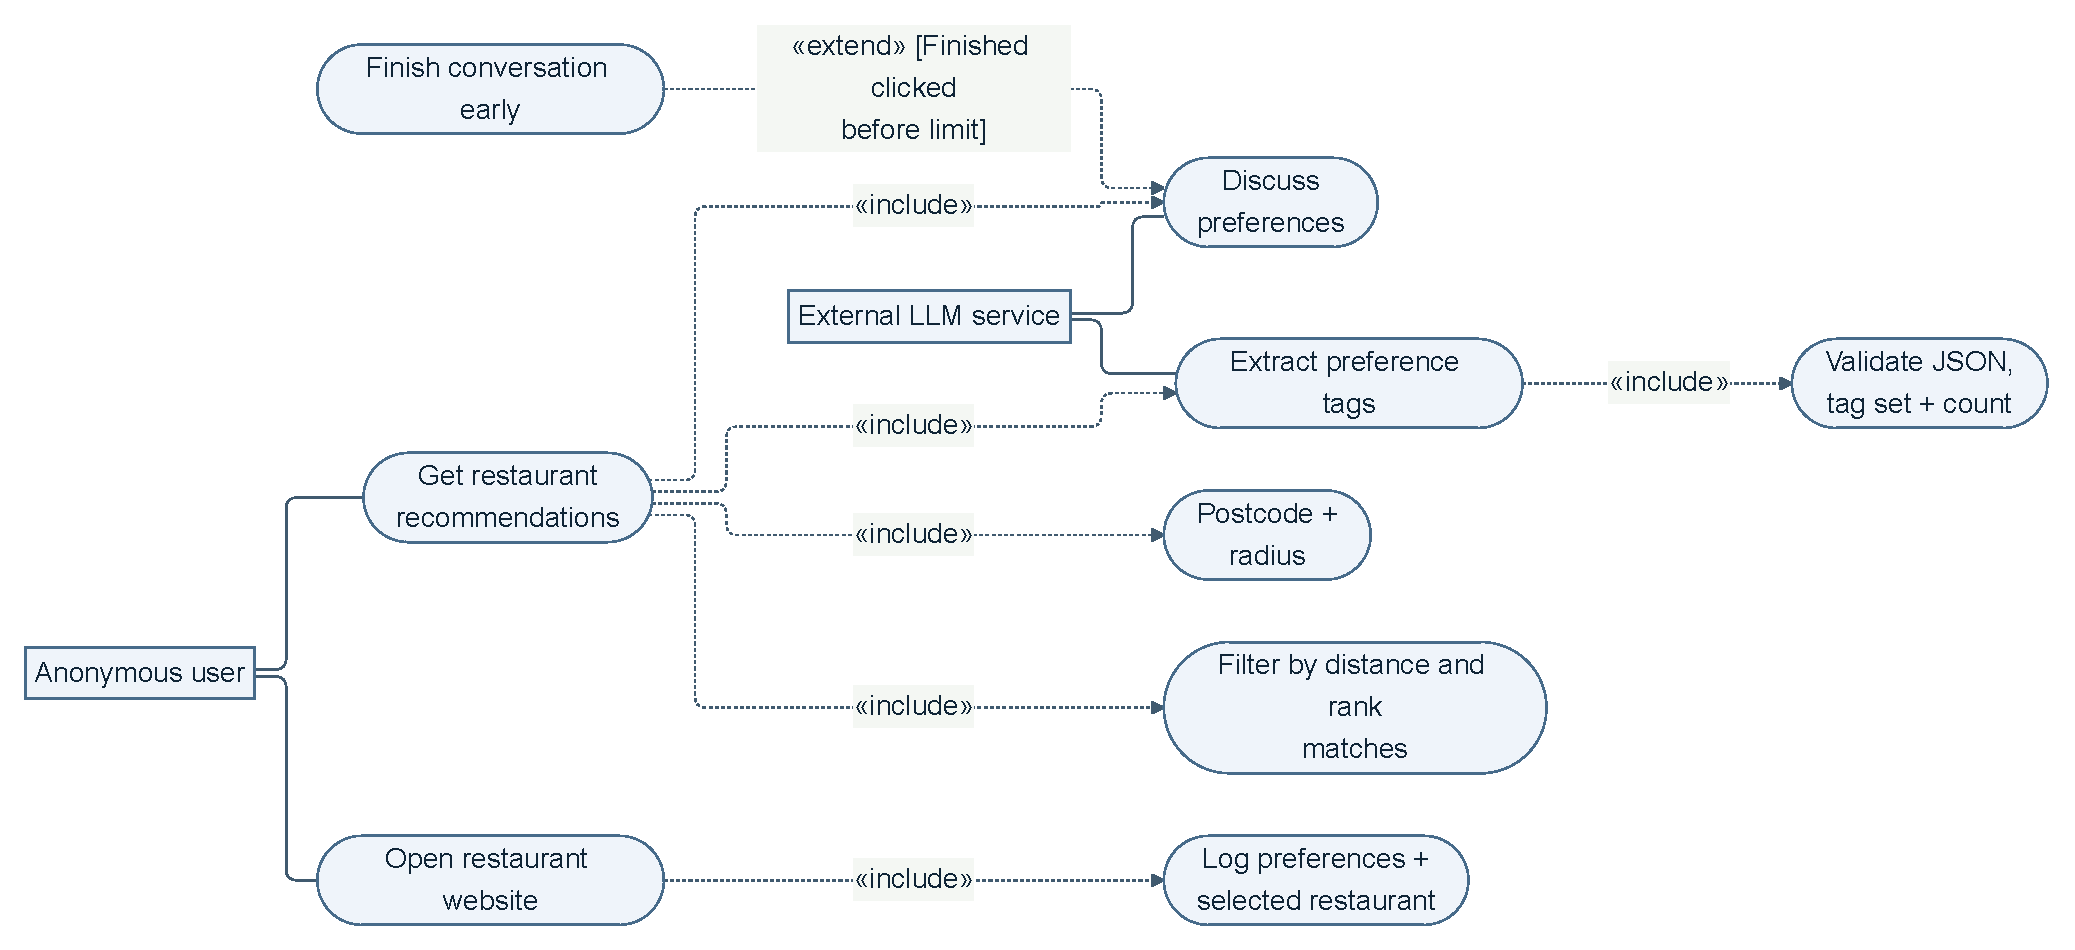
\includegraphics[width=514.00pt]{images/fig-085-user.pdf}
\captionof{figure}{Q1 --- Use cases and JSON-check activity (25 marks) --- anonymous user and supporting LLM view}\end{minipage}\par\smallskip








\par\smallskip\noindent\begin{minipage}{\linewidth}\centering
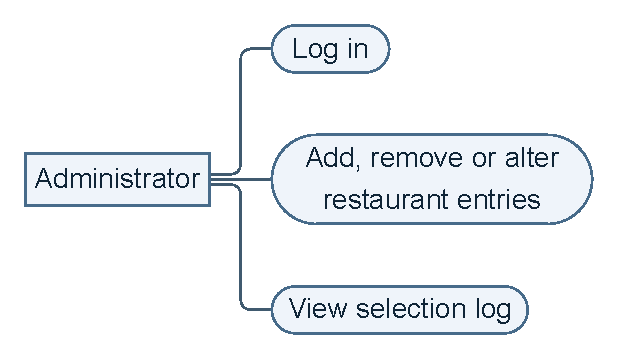
\includegraphics[width=173.80pt]{images/fig-085-admin.pdf}
\captionof{figure}{Q1 --- Use cases and JSON-check activity (25 marks) --- administrator view}\end{minipage}\par\smallskip

\begin{studycolumns}
\vspace{0pt}



Protected administrator actions require authentication; anonymous recommendations do not. Early finish is optional; reaching ten completed pairs also ends the conversation. Location/\allowbreak{}ranking steps belong to the successful flow; validation failure terminates that attempt before them. Recording a selection happens on a website click, not automatically for every displayed restaurant.

\textbf{(b)} \textbf{Schema assumption:} the LLM contract represents tags as a JSON array of strings (or an agreed object field holding that array). JSON validity alone does not ensure that the parsed shape is usable as a tag list.
\end{studycolumns}


\par\smallskip\noindent\begin{minipage}{\linewidth}\centering
{\scriptsize\textbf{Validate JSON, shape, count and fixed tag set}}\par\smallskip
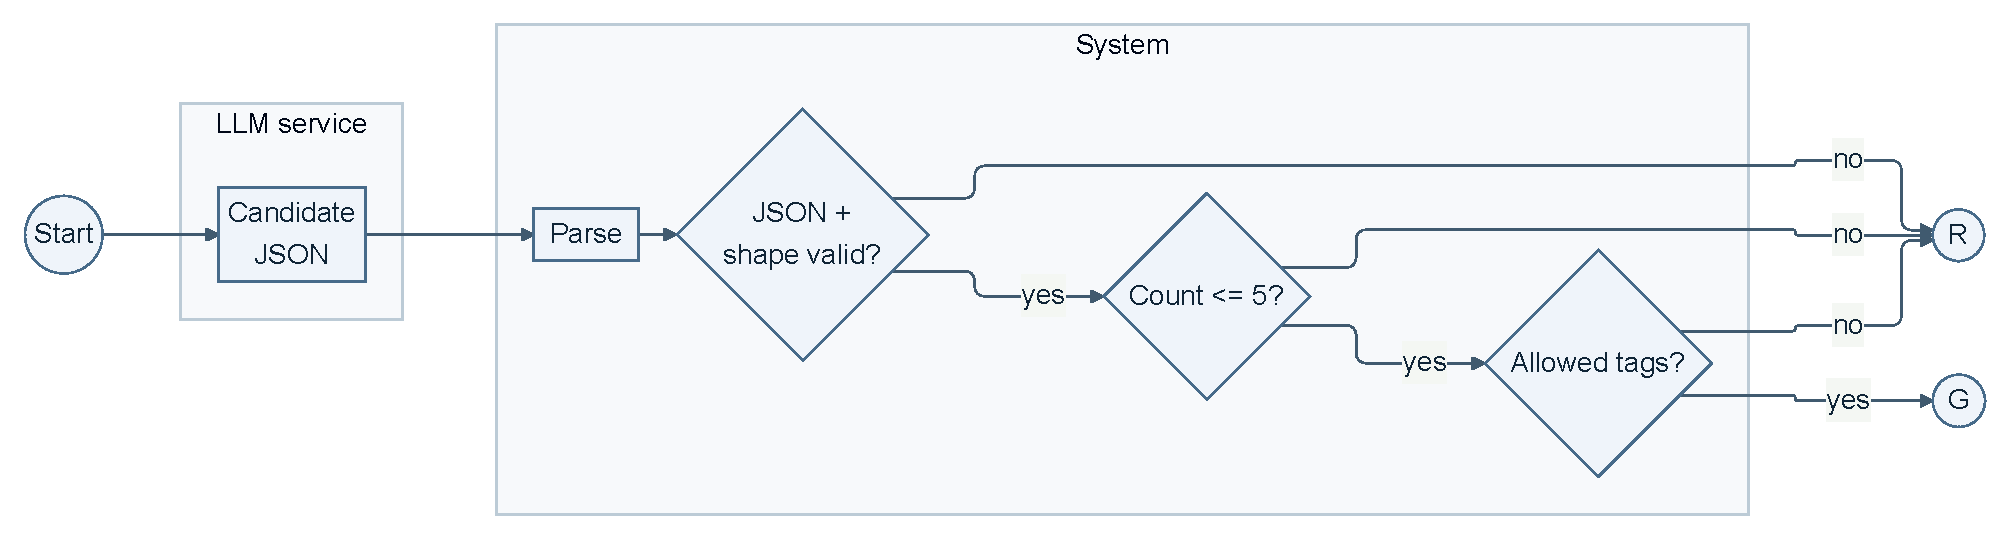
\includegraphics[width=514.00pt]{images/fig-086-a.pdf}\par\smallskip
{\scriptsize\textbf{Accept location input or offer restart}}\par\smallskip
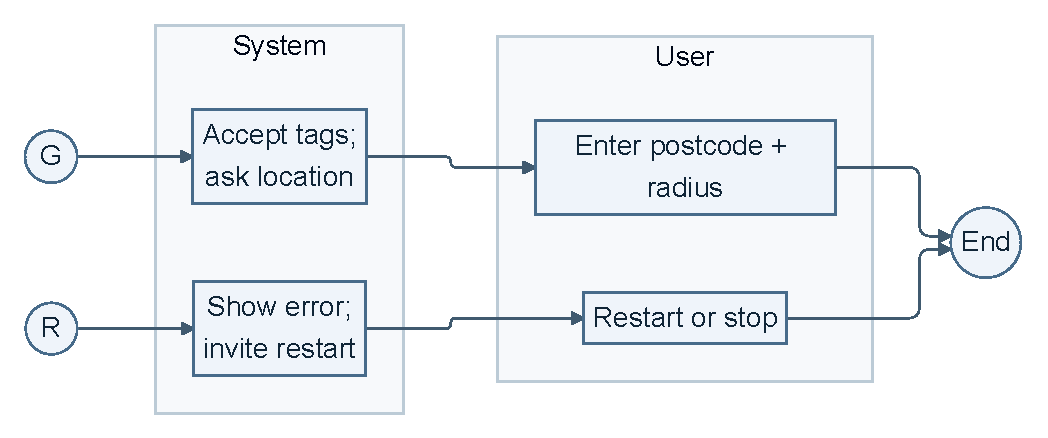
\includegraphics[width=268.00pt]{images/fig-086-b.pdf}\par\smallskip
\captionof{figure}{Q1 --- Use cases and JSON-check activity (25 marks) --- G = accepted tags; R = rejected candidate.}\end{minipage}\par\smallskip

\begin{studycolumns}
\vspace{0pt}




``Up to five'' supplies no minimum-one rule: do not reject an empty tag list unless a separate requirement establishes that rule. Duplicate-tag handling is unspecified; do not silently add a rejection requirement. Count entries before any optional deduplication so a six-entry response cannot evade the stated limit.

\needspace{4\baselineskip}
\subsection*{Q2 --- Recommendation classes, conversation states and Scrum (25 marks)}
\sectionlabel{h-q2--recommendation-classes-conversation-states-and-scrum-25-marks}
\textbf{(a) Recommendation-generation conceptual classes/\allowbreak{}stereotypes (8). (b) Conversation state machine (6). (c) Waterfall versus Agile when the tag set changes (5). (d) Two causes/\allowbreak{}remedies for frequently overrun sprints (6).}


\textbf{(a)}
\end{studycolumns}


\par\smallskip\noindent\begin{minipage}{\linewidth}\centering
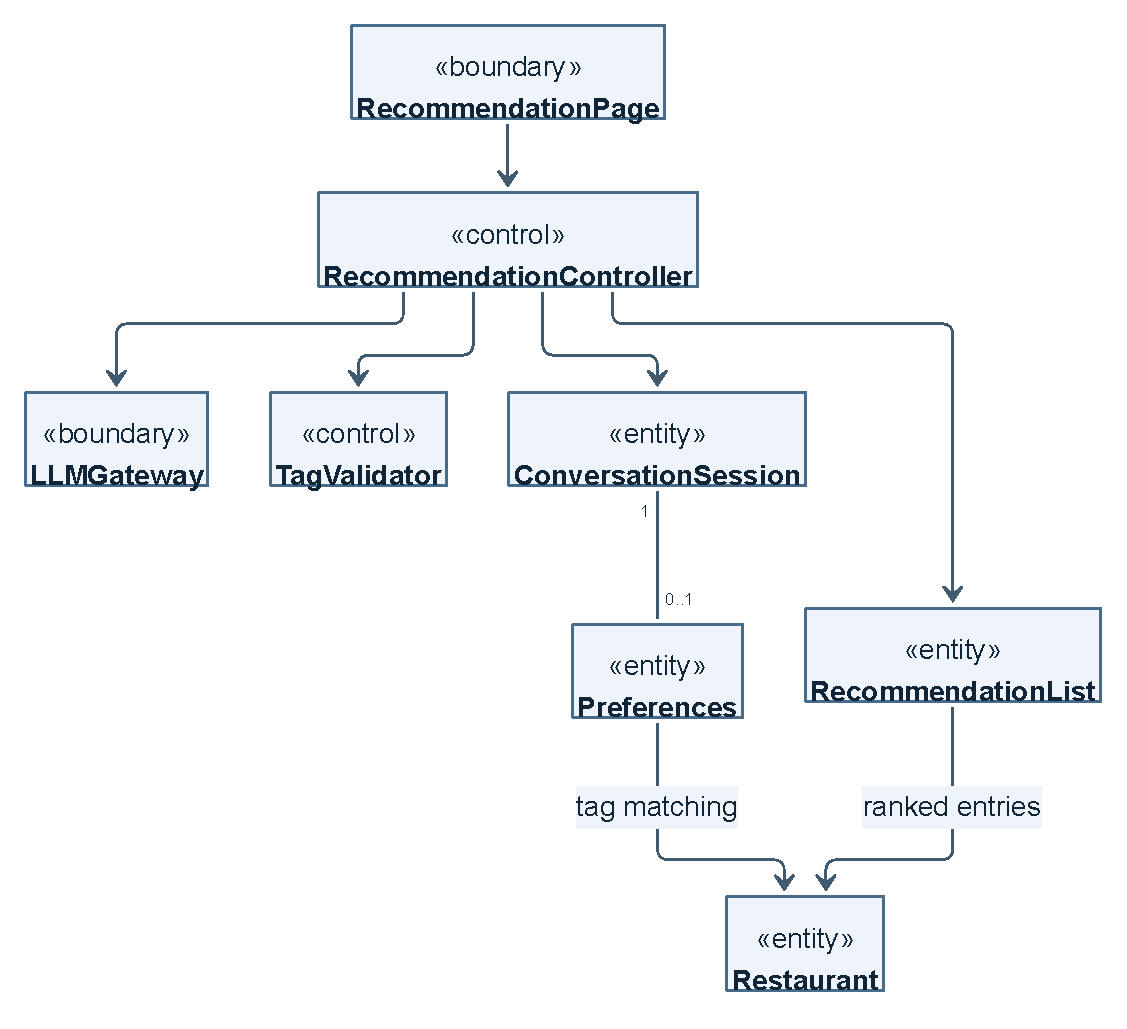
\includegraphics[width=306.81pt]{images/fig-087.pdf}
\captionof{figure}{Q2 --- Recommendation classes, conversation states and Scrum (25 marks)}\end{minipage}\par\smallskip



Postcode/\allowbreak{}radius belong to the recommendation request; preferences contain validated tags. No registered-user entity is required for anonymous use.

\textbf{(b)} Count \textbf{completed user/\allowbreak{}assistant pairs}, not individual messages. The limit is ten of each, not ten combined.




\par\smallskip\noindent\begin{minipage}{\linewidth}\centering
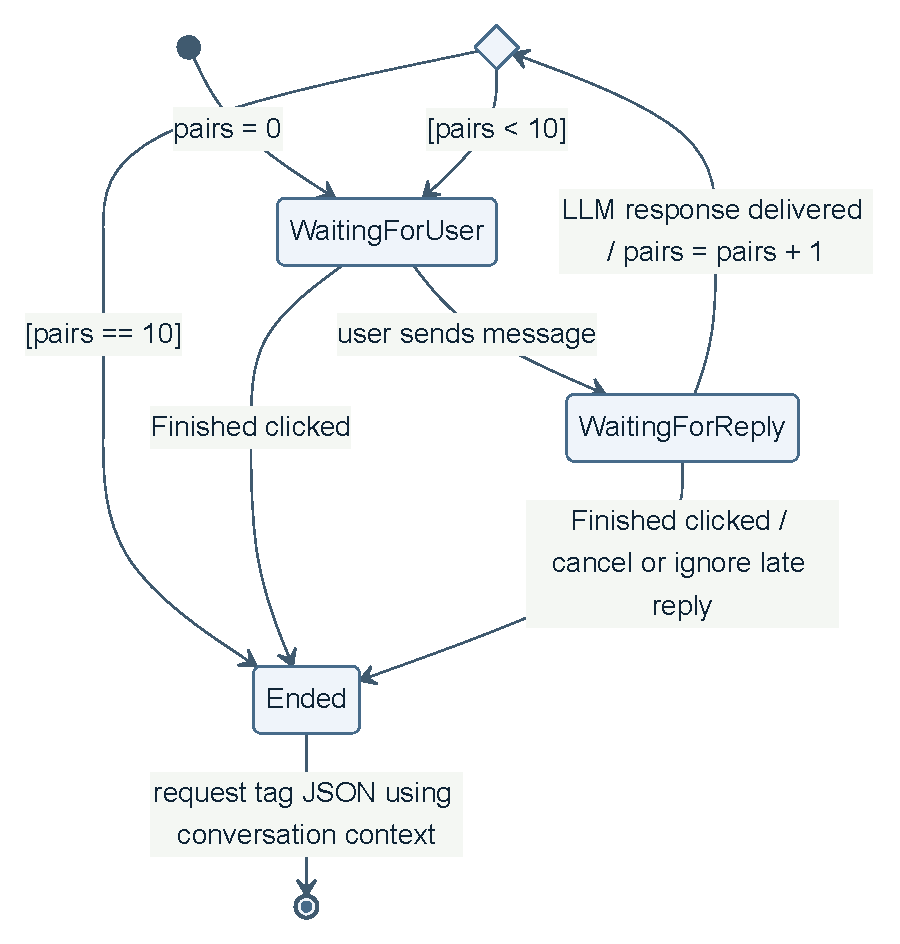
\includegraphics[width=253.00pt]{images/fig-088.pdf}
\captionof{figure}{Q2 --- Recommendation classes, conversation states and Scrum (25 marks)}\end{minipage}\par\smallskip

\begin{studycolumns}
\vspace{0pt}



Handling Finished while a reply is pending is a stated design choice; it must not reopen the ended conversation when a late reply arrives. Restart after invalid tag JSON starts a fresh session. JSON validation/\allowbreak{}recommendation are subsequent components, not extra conversation messages.

\textbf{(c)} Apply \hyperref[answer-waterfall]{W, p.\ \pageref{answer-waterfall}}. A tag-set change affects prompts, validators, restaurant data, UI and tests. Version/configure the vocabulary consistently; changing only the prompt is insufficient.

\textbf{(d)} Use \hyperref[answer-scrum]{S, p.\ \pageref{answer-scrum}}. Oversized/optimistic stories: split and select less work using actual capacity. Hidden LLM/API/integration or support work: investigate early, use doubles and budget support capacity. Replan unfinished work.

\end{studycolumns}
\Needspace{85pt}
\subsection*{Q3 --- Architecture and external LLM trade-offs (25 marks)}
\begin{studycolumns}
\sectionlabel{h-q3--architecture-and-external-llm-trade-offs-25-marks}
\textbf{(a) Architecture (3). (b) Detailed classes with attributes/\allowbreak{}methods (12). (c)(i) Two upsides/\allowbreak{}two downsides of self-hosting an LLM (4); (ii) two other responses to a hosted LLM advertising competitors (6).}


\textbf{(a)} Use client--server with layered application/\allowbreak{}domain services and an external LLM gateway. MVC can organise browser interaction: views display conversation/\allowbreak{}results, controllers accept inputs, and domain models/\allowbreak{}services hold conversation, tag-validation and recommendation rules. Keep the restaurant database, logging and administrator authorisation on the server; never trust unvalidated LLM output.

\textbf{(b)} Two views of one class model keep the diagram readable. \code{Session\allowbreak{}Controller} is the same class in both views; operations are shown in the view that uses them.
\end{studycolumns}


\par\smallskip\noindent\begin{minipage}{\linewidth}\centering
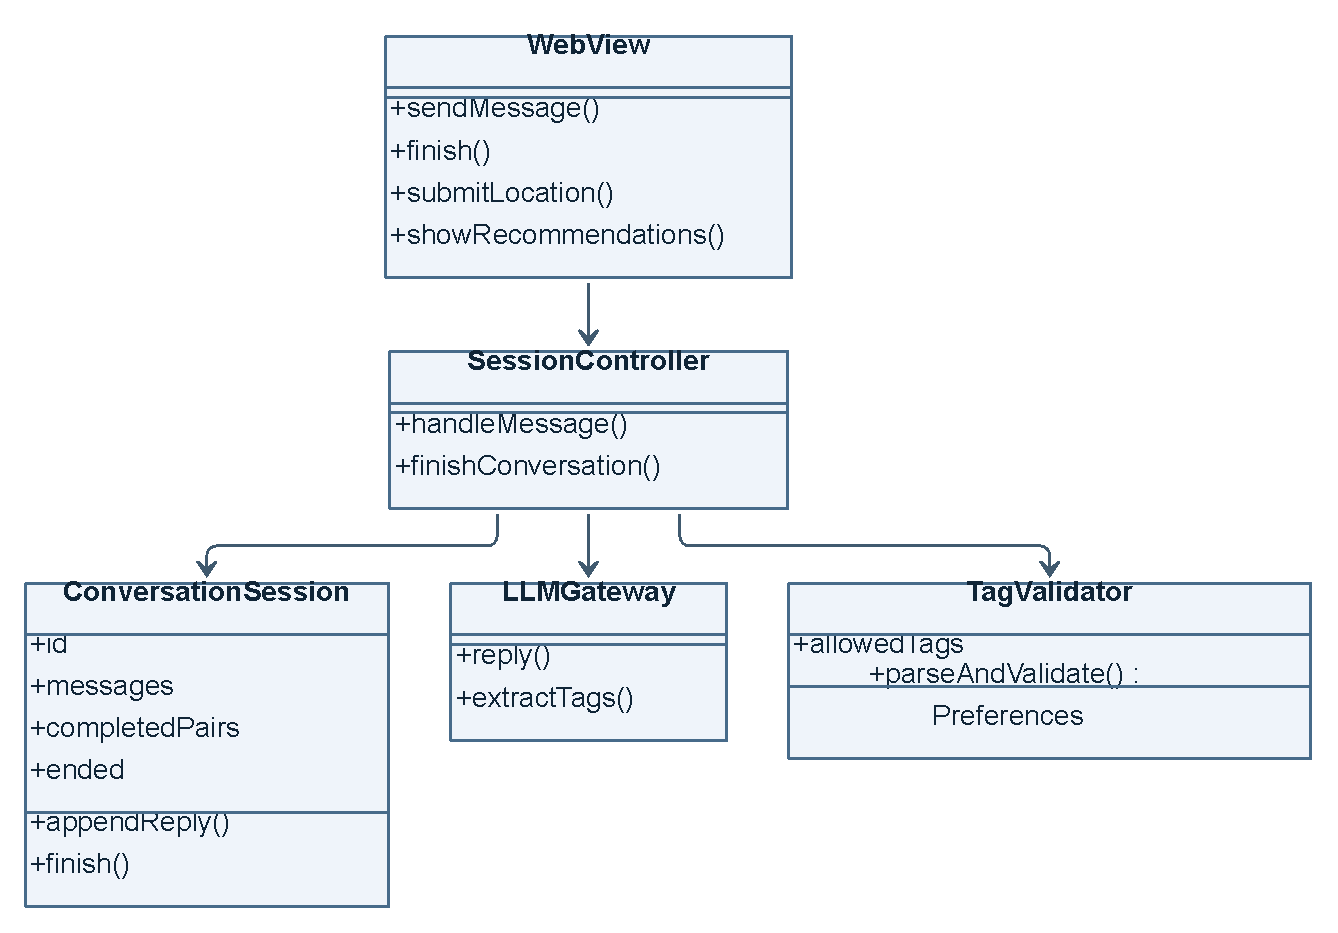
\includegraphics[width=376.64pt]{images/fig-089.pdf}
\captionof{figure}{Q3 --- Architecture and external LLM trade-offs (25 marks)}\end{minipage}\par\smallskip









\par\smallskip\noindent\begin{minipage}{\linewidth}\centering
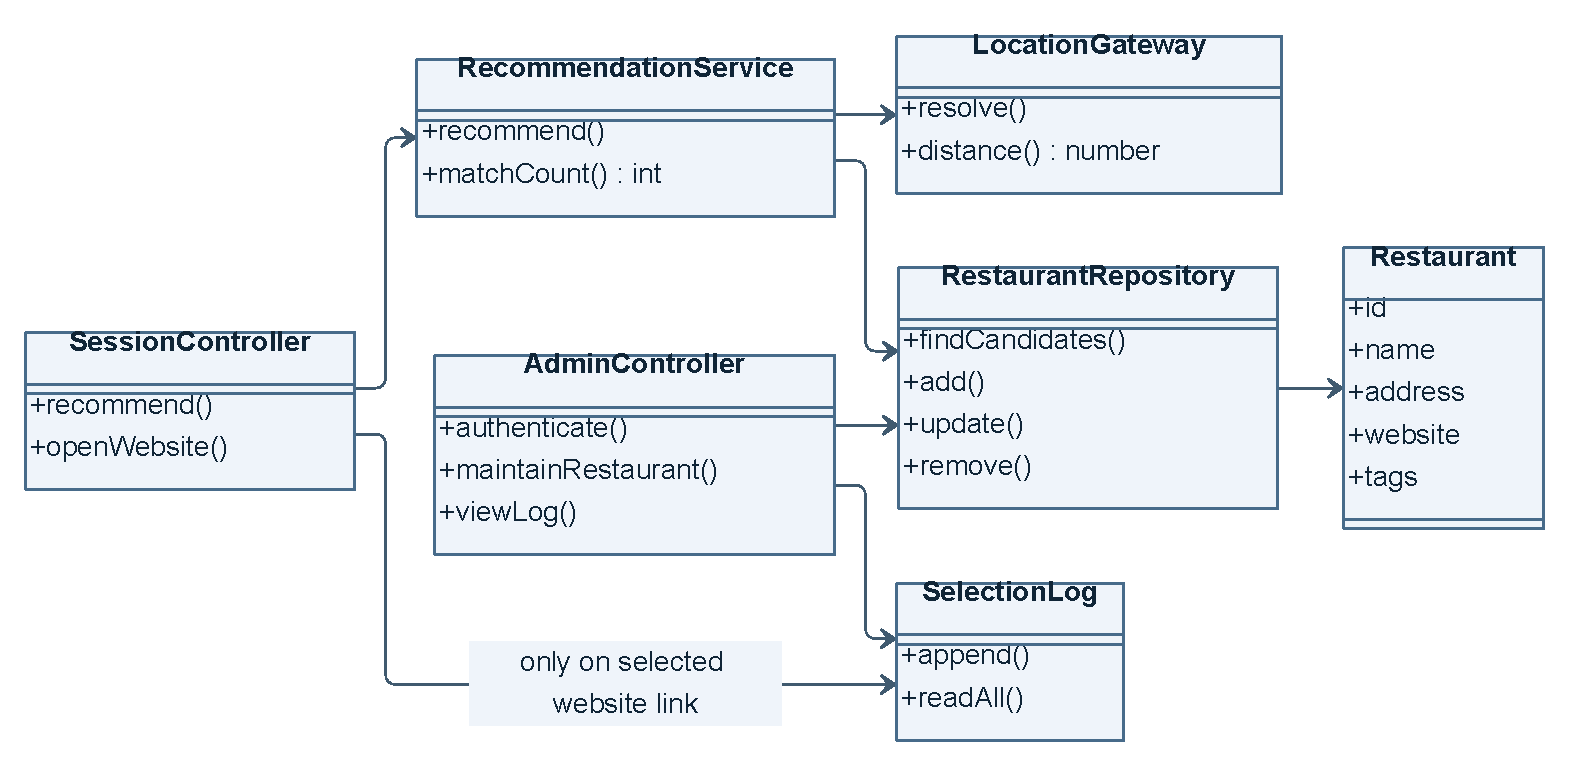
\includegraphics[width=441.76pt]{images/fig-090.pdf}
\captionof{figure}{Q3 --- Architecture and external LLM trade-offs (25 marks)}\end{minipage}\par\smallskip

\begin{studycolumns}
\vspace{0pt}





A server-side selection endpoint records the preferences/\allowbreak{}restaurant associated with that anonymous session, then redirects to the restaurant website. Domain algorithm: resolve location; retain restaurants with \code{distance \ensuremath{\leq} radius}; compute the number of matching preference tags; sort descending; display names and website links. Zero matches are not explicitly excluded. Tie ordering and distance calculation method are unspecified; declare any chosen policy. Location resolution is a proposed integration needed for distance calculation, distinct from Q4's initially format-only validator.

\textbf{(c)(i)} Self-hosting upsides: \textbf{control over model behaviour/\allowbreak{}version/\allowbreak{}customisation}, and \textbf{control over data handling with less dependence on a hosted provider's policies/\allowbreak{}availability}. Downsides: \textbf{compute/\allowbreak{}infrastructure cost}, and \textbf{operational/\allowbreak{}expertise burden} for serving, monitoring, updates, capacity and security. Self-hosting does not automatically deliver better accuracy or eliminate harmful outputs.

\textbf{(c)(ii)} Two approaches other than self-hosting:

\begin{enumerate}
\item \textbf{Switch to another externally hosted model/\allowbreak{}provider}, through the gateway, after testing against conversation and tag-extraction requirements. Establish service/\allowbreak{}content expectations and regression checks; avoid merely assuming every alternative behaves better.
\item \textbf{Add a server-side output-policy boundary.} Check user-visible replies for unwanted promotional content, block affected responses and request a constrained regeneration with bounded retries; provide a controlled error/\allowbreak{}fallback when checks fail. Keep tag extraction under strict structural/\allowbreak{}membership validation as well. A prompt instruction alone is not a reliable enforcement boundary, and valid JSON does not establish that freeform replies contain no advertising. Evaluate false positives/\allowbreak{}negatives and preserve the required conversation capability.
\end{enumerate}
\needspace{4\baselineskip}
\subsection*{Q4 --- Postcode/\allowbreak{}distance ECs, external API and internationalisation (25 marks)}
\sectionlabel{h-q4--postcodedistance-ecs-external-api-and-internationalisation-25-marks}
\textbf{Given:} \code{validate\allowbreak{}User\allowbreak{}Input(postcode,\allowbreak{} distance)} accepts a postcode string of six numerical digits and an integer distance from 0 to 100 km inclusive. \textbf{(a) ECs/\allowbreak{}assumptions (4). (b) Boundary triplets (4). (c) Defensive suite (8). (d)(i) EC changes when a public API confirms a real Singapore building (3); (ii) two complications for comprehensive tests (4). (e) Adaptation to multiple countries (2).}


\textbf{(a)} Assume ``numerical digits'' means ASCII \code{0}--\code{9}, retain leading zeroes, do not trim/\allowbreak{}coerce invalid inputs silently, and initially check \textbf{syntax only}, not real-building existence. The function contract already gives string/\allowbreak{}integer argument types; non-string/\allowbreak{}non-integer inputs are extra defensive-interface cases if the implementation permits them.
\end{studycolumns}


{\fontsize{8.5}{9.8}\selectfont
\begin{longtable}{L{\dimexpr 0.23363\linewidth-5.61pt\relax}L{\dimexpr 0.31394\linewidth-7.53pt\relax}L{\dimexpr 0.45243\linewidth-10.86pt\relax}}
\toprule
\rowcolor{ice}\textbf{Input} & \textbf{Valid EC} & \textbf{Invalid ECs} \\
\midrule\endfirsthead
\toprule\rowcolor{ice}\textbf{Input} & \textbf{Valid EC} & \textbf{Invalid ECs} \\
\midrule\endhead
\multicolumn{3}{r}{\scriptsize Continued on next page}\\\endfoot
\bottomrule\endlastfoot
Postcode & Exactly six ASCII digits: \code{[0-\allowbreak{}9]\{6\}} & Length other than six; length six with at least one non-digit (including non-ASCII digits) \\
Distance & Integer \code{0 \ensuremath{\leq} d \ensuremath{\leq} 100} & Integer \code{d < 0}; integer \code{d >\allowbreak{} 100} \\
\end{longtable}
}

\begin{studycolumns}
\vspace{0pt}

The postcode invalid classes are disjoint as defined. \code{000000} and \code{999999} are syntactically valid even if they do not identify buildings. Postcode is not an integer range from 100000 to 999999.

\textbf{(b)} Distance triplets: \code{\ensuremath{-}1,\allowbreak{} 0,\allowbreak{} 1} and \code{99,\allowbreak{} 100,\allowbreak{} 101}. Postcode \textbf{length} triplet: length \code{5,\allowbreak{} 6,\allowbreak{} 7}, e.g. \code{00000}, \code{000000}, \code{0000000}. Character membership is a discrete format rule; use a six-character string containing a letter/\allowbreak{}space rather than inventing an overall numeric postcode boundary.

\textbf{(c)} Reset/\allowbreak{}isolate each test. ``Accept'' means this validator returns acceptance; it does not promise that later geocoding/\allowbreak{}recommendation will succeed.
\end{studycolumns}


{\fontsize{8.5}{9.8}\selectfont
\begin{longtable}{L{\dimexpr 0.28067\linewidth-6.74pt\relax}L{\dimexpr 0.28067\linewidth-6.74pt\relax}L{\dimexpr 0.43866\linewidth-10.53pt\relax}}
\toprule
\rowcolor{ice}\textbf{Postcode string} & \textbf{Distance (km)} & \textbf{Expected /\allowbreak{} purpose} \\
\midrule\endfirsthead
\toprule\rowcolor{ice}\textbf{Postcode string} & \textbf{Distance (km)} & \textbf{Expected /\allowbreak{} purpose} \\
\midrule\endhead
\multicolumn{3}{r}{\scriptsize Continued on next page}\\\endfoot
\bottomrule\endlastfoot
\code{612345} & 50 & Accept --- baseline \\
\code{000000} & 50 & Accept --- leading zeroes, syntax only \\
\code{999999} & 50 & Accept --- six digits, syntax only \\
\code{612345} & 0 & Accept --- lower distance boundary \\
\code{612345} & 1 & Accept --- lower valid neighbour \\
\code{612345} & 99 & Accept --- upper valid neighbour \\
\code{612345} & 100 & Accept --- upper distance boundary \\
\code{612345} & \ensuremath{-}1 & Reject --- distance below minimum \\
\code{612345} & 101 & Reject --- distance above maximum \\
\code{00000} & 50 & Reject --- five characters \\
\code{0000000} & 50 & Reject --- seven characters \\
\code{12345a} & 50 & Reject --- six characters with non-digit \\
\code{123 45} & 50 & Reject --- embedded space \\
\code{[six full-\allowbreak{}width digits]} & 50 & Reject --- non-ASCII digits under stated assumption \\
empty string & 50 & Reject --- wrong length \\
\end{longtable}
}

\begin{studycolumns}
\vspace{0pt}

All rejected rows contain exactly one invalid parameter. If runtime types are not enforced, add type-check tests such as fractional distance and a numeric rather than string postcode, with explicit rejection policy.

\textbf{(d)(i)} Split the old valid-syntax postcode class into \textbf{API-confirmed real-building postcodes} and \textbf{well-formed postcodes confirmed not to identify a building}. Keep malformed classes. Timeout, unavailable service, malformed API response or rate limiting is a dependency-failure outcome, not proof that the postcode is invalid. Define fail/\allowbreak{}retry/\allowbreak{}error behaviour explicitly.

\textbf{(d)(ii)} Two complications: \textbf{changing external data}, so a postcode's building association/\allowbreak{}validity may change and make hard-coded oracles stale; \textbf{nondeterministic service behaviour}, including network failures, latency, limits and unexpected response formats. Use versioned fixtures/\allowbreak{}test doubles for deterministic unit/\allowbreak{}contract cases and a smaller controlled live integration suite with recorded expectations. Exercise confirmed-valid, confirmed-absent and each failure response; do not claim that a mocked suite verifies live API availability.

\textbf{(e)} Add a country identifier or country-specific validation policy: \code{validate\allowbreak{}User\allowbreak{}Input(country\allowbreak{}Code,\allowbreak{} postcode,\allowbreak{} distance)}. Select the appropriate format and, where required, country-specific lookup service. Preserve postcodes as strings because countries may use letters, spaces and leading zeroes. Define normalisation and accepted formats per country and parameterise tests; do not impose Singapore's six-digit rule globally.
\end{studycolumns}
